\chapter{MARCO TEÓRICO}

\section{Conceptos básicos}
\subsection{Lenguaje de programación}
Los lenguajes de programación son notaciones que describen los cálculos a las personas y las máquinas. Nuestra percepción del mundo en que vivimos depende de los lenguajes de programación, ya que todo el software que se ejecuta en todas las computadoras se escribió en algún lenguaje de programación \cite{aho2008compiladores}.

\subsection{Código fuente}
El código fuente de un programa está escrito por un programador en algún lenguaje de programación, pero en este primer estado no es directamente ejecutable por la computadora, sino que debe ser traducido a otro lenguaje o código binario, así será más fácil para la máquina interpretarlo. Para esta traducción se usan los llamados compiladores, ensambladores, intérpretes y otros sistemas de traducción \cite{wiki:Source_Code}.

\section{Conceptos de compiladores}
\subsection{Procesador de lenguaje}
Un procesador de lenguaje (figura 2.1) también llamado compilador es un programa que puede leer un programa en un lenguaje y traducirlo en un programa equivalente en otro lenguaje. Una función importante del compilador es reportar cualquier error en el programa fuente que detecte durante el proceso de traducción \cite{aho2008compiladores}.
\begin{figure}[htb]
\centering
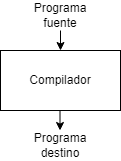
\includegraphics[scale=0.8]{imagenes/compilador}
\caption{Compilador}
\end{figure}
El proceso de compilación opera como una secuencia de fases con las cuales transforma un programa fuente en otro como se muestra en la figura 2.2.
\begin{figure}[htb]
\centering
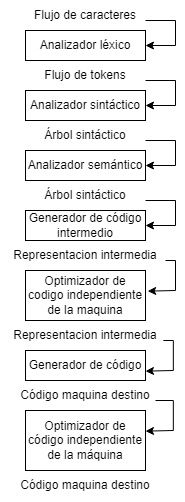
\includegraphics[scale=0.8]{imagenes/fasesCompilador}
\caption{Fases de un compilador}
\end{figure}
En el presente trabajo de investigación, solo es de interés de la investigación cubrir los conceptos y teoría hasta el análisis semántico.
\subsection{Análisis Léxico}
En la primera fase de un compilador. El analizador de léxico lee el flujo de caracteres que componen el programa fuente y los agrupa en secuencias significativas, conocidas como lexemas. Para cada lexema, el analizador léxico produce como salida un token de la forma:
\begin{center}
[nombre-token, valor-atributo]
\end{center}
estos lexemas son los que pasaran a la fase siguiente fase, el análisis de la sintaxis. En el token, el primer componente nombre-token es un símbolo abstracto que se utiliza durante el análisis sintáctico, y el segundo componente valor-atributo apunta a una entrada en la tabla de símbolos para este token. La información de la entrada en la tabla de símbolos se necesita para el análisis semántico y la generación de código.
Por ejemplo, suponga que un programa fuente contiene la instrucción de asignación:
\begin{center}
    posicion = inicial + velocidad * 60
\end{center}
Los caracteres en esta asignación podrían agruparse en los siguientes lexemas y mapearse a los siguientes tokens que se pasan al analizador sintáctico:
\begin{enumerate}
    \item posicion es un lexema que se asigna a un token [id, 1], en donde id es un símbolo abstracto que representa la palabra identificador y 1 apunta a la entrada en la tabla de símbolos para posicion. La entrada en la tabla de símbolos para un identificador contiene información acerca de éste, como su nombre y tipo.
    \item  El símbolo de asignación = es un lexema que se asigna al token [=]. Como este token no necesita un valor-atributo, hemos omitido el segundo componente. Podríamos haber utilizado cualquier símbolo abstracto como asignar para el nombre-token, pero por conveniencia de notación hemos optado por usar el mismo lexema como el nombre para el símbolo abstracto.
    \item inicial es un lexema que se asigna al token [id, 2], en donde 2 apunta a la entrada en la tabla de símbolos para inicial.
    \item + es un lexema que se asigna al token [+].
    \item velocidad es un lexema que se asigna al token [id, 3], en donde 3 apunta a la entrada en la tabla de símbolos para velocidad.
    \item * es un lexema que se asigna al token [*].
    \item 60 es un lexema que se asigna al token [60].
\end{enumerate}
El analizador léxico ignora los espacios en blanco que separan a los lexemas.
\begin{center}
[id, 1] [=] [id, 2] [+] [id, 3] [*] [60] 
\end{center}
En esta representación, los nombres de los tokens =, + y * son símbolos abstractos para los operadores de asignación, suma y multiplicación, respectivamente.
\subsection{Análisis Sintáctico}
La segunda fase del compilador es el análisis sintáctico o parsing. El parser (analizador sintáctico) utiliza los primeros componentes de los tokens producidos por el analizador de léxico para crear una representación intermedia en forma de árbol que describa la estructura gramatical del flujo de tokens. Una representación típica es el árbol sintáctico, en el cual cada nodo interior representa una operación y los hijos del nodo representan los argumentos de la operación.
En la figura 2.3 se muestra un árbol sintáctico para el flujo de tokens como salida del analizador sintáctico.
\subsection{Análisis Semántico}
El analizador semántico utiliza el árbol sintáctico y la información en la tabla de símbolos para comprobar la consistencia semántica del programa fuente con la definición del lenguaje. También recopila información sobre el tipo y la guarda, ya sea en el árbol sintáctico o en la tabla de símbolos, para usarla más tarde durante la generación de código intermedio.
Una parte importante del análisis semántico es la comprobación (verificación) de tipos, en donde el compilador verifica que cada operador tenga operando que coincidan. Por ejemplo, muchas definiciones de lenguajes de programación requieren que el índice de un arreglo sea entero; el compilador debe reportar un error si se utiliza un número de punto flotante para indexar el arreglo.
Observe en la figura 2.3 que la salida del
analizador semántico tiene un nodo adicional para el operador inttofloat
\begin{figure}[htb]
\centering
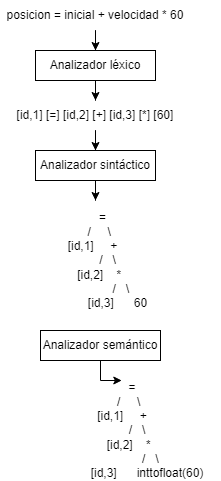
\includegraphics[scale=0.8]{imagenes/traduccionDeAsignacion}
\caption{Traducción de una asignación}
\end{figure}
\section{Representación de código fuente}

\subsection{Arboles}
En ciencias de la computación y en informática, un árbol es un tipo abstracto de datos ampliamente usado que imita la estructura jerárquica de un árbol, con un valor en la raíz y subárboles con un nodo padre, representado como un conjunto de nodos enlazados.\\
Una estructura de datos de árbol se puede definir de forma recursiva como una colección de nodos a partir de un nodo raíz, donde cada nodo es una estructura de datos con un valor, junto con una lista de referencias a los nodos, con la condición de que ninguna referencia esté duplicada ni que ningún nodo apunte a la raíz.

\subsection{Árboles de sintaxis abstracta}
Las estructuras de datos basadas en árboles se hicieron muy populares en el campo del desarrollo de compiladores: cada vez que se envía un archivo que contiene el código fuente al compilador, se realizan varios pasos antes de que se puedan generar las instrucciones de la máquina. El código tiene que ser tokenizado por un Lexer primero: separa el flujo de entrada en tokens individuales y los pasa al analizador, que utiliza una gramática libre de contexto del lenguaje de programación para construir una representación de código intermedio, un llamado árbol de análisis.
Cada token encontrado por el lexer está representado por un nodo en el árbol de análisis. No todos los tokens (nodos) tienen un valor semántico: algunos tokens, por ejemplo, paréntesis y punto y coma, son puramente sintácticos. Por lo tanto, puede omitirse. La estructura de datos resultante se denomina árbol de sintaxis abstracta (AST).
Ahora que el código fuente se representa como un árbol, se puede analizar de una forma más sofisticada manera que al analizar el flujo de token plano: el árbol se puede recorrer o buscar de varias maneras (por ejemplo, pos-orden, pre-orden, búsqueda profundidad, etc.) \cite{ChangeDistiller}.


\section{Conceptos de algorítmica}
\subsection{Programación dinámica}
La programación dinámica es una técnica matemática que se utiliza para la solución de problemas matemáticos seleccionados, en los cuales se toma un serie de decisiones en forma secuencial.

\subsection{Distancia de edición}
La distancia edición o distancia entre palabras es el número mínimo de operaciones requeridas para transformar una cadena de caracteres en otra, se usa ampliamente en teoría de la información y ciencias de la computación. Se entiende por operación, bien una inserción, eliminación o la sustitución de un carácter. Esta distancia recibe ese nombre en honor al científico ruso Vladimir Levenshtein, quien se ocupó de esta distancia en 1965. Es útil en programas que determinan cuán similares son dos cadenas de caracteres, como es el caso de los correctores ortográficos.

\subsection{Distancia de edición del árbol}
La distancia de edición del árbol se define como la secuencia de costos mínimos de operaciones de edición de nodos que transforman un árbol en otro. Las operaciones consisten en eliminar, agregar y modificar nodos del árbol.

\subsection{Algoritmos utilizados para la detección de similitud entre códigos fuente}
\cite{10.1145/3313290} Identificó diferentes algoritmos a continuación se mencionan algunos de ellos:

\begin{itemize}
    \item Recuento de atributos
    \item Huella digital
    \item Coincidencia de cadena
    \item Texto base
    \item Estructura base
    \item Estilo
    \item Semántico
    \item N-gramas
    \item Árboles
    \item Grafos
\end{itemize}

Algunos de estos fueron inventados en la década de 1980. También hace mención a que los enfoques basados en estructuras son mucho mejores y que la mayoría de las herramientas de detección de similitud combinan más de un tipo de algoritmo.

\section{Conceptos de ofuscación de código fuente}
\subsection{Plagio de código fuente}
\cite{wiki:Plagiarism} La Real Academia Española define como plagio a la acción de copiar en lo sustancial obras ajenas, dándolas como propias.

El plagio de código fuente consiste en utilizar el código fuente de otra persona y adjudicarse como propio.

\subsection{Ofuscación}
La ofuscación se refiere a encubrir el significado de una comunicación haciéndola más confusa y complicada de interpretar \cite{wiki:Obfuscation_(software)}.

\subsection{Ofuscación de código fuente}
En computación, la ofuscación se refiere al acto deliberado de realizar un cambio no destructivo, ya sea en el código fuente de un programa informático, en el código intermedio (bytecodes) o en el código máquina cuando el programa está en forma compilada o binaria. Es decir, se cambia el código se enrevesa manteniendo el funcionamiento original, para dificultar su entendimiento. De esta forma se dificultan los intentos de ingeniería inversa y desensamblado que tienen la intención de obtener una forma de código fuente cercana a la forma original \cite{wiki:Obfuscation_(software)}.

\subsection{Métodos de ofuscación de código fuente}
Existen muchos métodos de ofuscación utilizados por estudiantes para ocultar la similitud a continuación se mencionan algunos:
\begin{itemize}
    \item \cite{article3} Mencionan cambios visuales en el formato del código, por lo que parece diferente a primera vista, esto generalmente incluye la modificación de espacios en blanco como sangrías, espacios, nuevas líneas, etc.
    \item \cite{article3} Mencionan cambios en los comentarios del código.
    \item \cite{donaldson1981plagiarism} Mencionan el cambio de los nombres de los identificadores. como nombres de variables, nombres de constantes, nombres de funciones, nombres de clases, etc.
    \item \cite{donaldson1981plagiarism} Mencionan reordenar las líneas del código para las que el pedido no marca ninguna diferencia. Estos incluyen cambiar el orden de las declaraciones de variables, cambiando el orden de las declaraciones dentro de bloques de código como funciones, re ordenación de bloques de código o funciones, re ordenación de clases internas, etc.
\end{itemize}
\subsection{Detección léxica}
Las técnicas y herramientas para computar las diferencias textuales entre documentos son bien conocidas y aprobadas. Sin embargo, las herramientas existentes como GNU diff tratan con información plana, en lugar de jerárquica. Por lo general, calculan una lista de líneas que deben cambiarse, insertarse o eliminarse para que un primer documento coincida con el segundo. \cite{ChangeDistiller}.